\question{Криволинейный интеграл 2-го рода как работа силы вдоль пути. Определение, вычисление и свойства.}

Пусть дана простая дуга \(\breve{AB}\) и некоторая сила \(\vec{F}(P, Q)\), где
\(P = P(x, y)\), \(Q = Q(x, y)\) это некоторые функции, зависящие от координат.

Построим интеграл:
\begin{enumerate}
  \item Введем ДПСК
  \item Вычислим среднюю элементарную работу \(\dd A\) вдоль элемента дуги
  \(\dd l\), а потом просуммируем все полученные элементарные работы:
  
  \begin{twocolumns}
    \begin{align*}
      \dd A = \vec{F} \vec{\dd s} = (P, Q) \cdot (\dd x, \dd y) \\
      A = \int_{AB} \dd A = \int_{AB} P(x, y) \dd x + Q(x, y) \dd y
    \end{align*}
    \columnbreak

    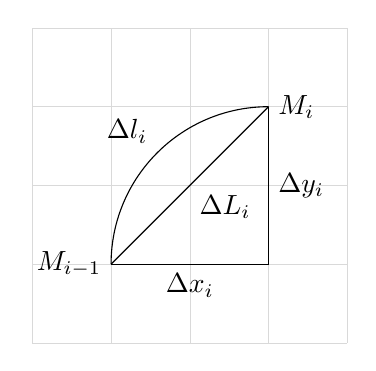
\begin{tikzpicture}  
  \draw[very thin, gray!30, step = 1cm] (0, 0) grid (4, 4);
  \draw (1, 1) -- (3, 1) -- (3, 3);
  \draw (3, 3) arc (90:180:2) node[midway, above left] {\(\Delta l_{i}\)};
  \draw (1, 1) -- (3, 3) node[midway, below right] {\(\Delta L_{i}\)};

  \draw node[below] at (2, 1) {\(\Delta x_{i}\)};
  \draw node[right] at (3, 2) {\(\Delta y_{i}\)};
  \draw node[left] at (1, 1) {\(M_{i - 1}\)};
  \draw node[right] at (3, 3) {\(M_{i}\)};
\end{tikzpicture}

  \end{twocolumns}

  \item Получили криволинейный интеграл 2-ого рода.
\end{enumerate}

\begin{remark}
  Можно рассматривать действие силы в каждом координатном направлении
  (в проекциях):

  \begin{align*}
    A_{x} = \int_{AB} P(x, y) \dd x \qquad
    A_{y} = \int_{AB} Q(x, y) \dd y
  \end{align*}

  поэтому криволинейный интеграл 2-ого рода иногда называют криволинейным
  интегралов в проекциях.
\end{remark}

\begin{remark}
  О математическом определении

  Криволинейный интеграл можно определить математически (дробление, составление
  интегральных сумм, переход к пределу, а затем и к интегралу), для этого нужно
  рассмотреть проекции на оси координат. В каждой из проекций получится
  криволинейный интеграл первого рода.
\end{remark}

\begin{remark}\label{curve-int-2-calc}
  О вычислении

  Параметризуем дугу и сведем все к определенному интегралу:

  \begin{align*}
    \int_{AB} P(x, y) \dd x + Q(x, y) \dd y \\
    \begin{cases}
      x = \phi(t) \implies \dd x = \phi'(t) \dd t \\
      y = \psi(t) \implies \dd y = \psi'(t) \dd t \\
      t \in [t_{1}, t_{2}] \iff A \to B
    \end{cases}
    \\
    \int_{t_{1}}^{t_{2}}
      P \Big( \phi(t), \psi(t) \Big) \phi'(t) \dd t
      + Q \Big( \phi(t), \psi(t) \Big) \psi'(t) \dd t
  \end{align*}
\end{remark}

\begin{remark}
  Криволинейный интеграл 2-ого рода (в отличие от криволинейного интеграла
  1-ого рода) зависит от направления обхода:

  \begin{align*}
    \int_{AB} P \dd x + Q \dd y = -\int_{BA} P \dd x + Q \dd y
  \end{align*}

  Остальные его свойства совпадают со свойствами определенного интеграла.
\end{remark}

